\documentclass[10pt]{article}

\usepackage{graphicx}
\usepackage{amsmath}
\usepackage{amssymb}
\usepackage{mathtools}
\usepackage{etoolbox}
\usepackage{booktabs}
\usepackage[parfill]{parskip}
\usepackage[numbers]{natbib}
\usepackage{float}
\usepackage{graphicx}
\usepackage{geometry}
\usepackage{multicol}
\usepackage{caption}
\usepackage{url}
% \usepackage[T1,T2A]{fontenc}
% \usepackage{lmodern}
% \usepackage[utf8]{inputenc}
% \usepackage[russian,english]{babel}
% 
% \renewcommand{\thesection}{\bfseries\arabic{section}}
% \renewcommand{\thesubsection}{\bfseries\arabic{subsection}}
% \renewcommand{\thesubsubsection}{\bfseries\arabic{subsubsection}}

\newcommand\mgin{0.5in}
\geometry{
    left=\mgin,
    right=\mgin,
    bottom=\mgin,
    top=\mgin
}

\usepackage[outdir=./eps2pdf/]{epstopdf}
\graphicspath{
  {../figures/}
  {../figures/goals/}
  {../figures/light_data/}
  {../figures/attenuation/}
}


% Define multicolumn figure-like environment
% from http://tex.stackexchange.com/questions/12262/multicol-and-figures
\newenvironment{mcfig}
    {\par\medskip\noindent\minipage{\linewidth}}
    {\endminipage\par\medskip}

% Define error function for math mode
\newcommand{\erf}{\mbox{erf}}
% Sign function
\newcommand{\sign}{\mbox{sign}}
% Natural numbers
\newcommand\NN{\mathbb{N}}
% Real numbers
\newcommand\RR{\mathbb{R}}
% Complex numbers
\newcommand\CC{\mathbb{C}}
% Curly B for basis
\newcommand\BB{\mathcal{B}}
% Curly D for diagonal dominance quantity
\newcommand\DD{\mathcal{D}}
\newcommand\QQ{\mathcal{Q}}
% Norm
\newcommand\norm[1]{\left\lVert #1 \right\rVert}
% Uniform Norm
\newcommand\unorm[1]{\left\lVert #1 \right\rVert_\infty}
% Inner Product
\newcommand\ip[1]{\left\langle #1 \right\rangle}
% Absolute value
\newcommand\abs[1]{\left| #1 \right|}
% Complex Conjugate
\newcommand\conj\overline
% Partial derivative
\newcommand\pd[2]{\frac{\partial #1}{\partial #2}}
% Iteration superscript w/ parentheses
\newcommand{\iter}[1]{^{(#1)}}
% Disable paragraph indentation
\setlength{\parindent}{0pt}
% End of proof
\newcommand\qed{\hfill$\blacksquare$\hspace{0.5in}}

% Domain
\newcommand\xmin{x_{\mbox{min}}}
\newcommand\xmax{x_{\mbox{max}}}
\newcommand\ymin{y_{\mbox{min}}}
\newcommand\ymax{y_{\mbox{max}}}
\newcommand\zmin{z_{\mbox{min}}}
\newcommand\zmax{z_{\mbox{max}}}

% Number this equation
\newcommand\eqnum{\addtocounter{equation}{1}\tag{\theequation}}

% Boldface vectors
\renewcommand\vec{\mathbf}

% arara: pdflatex
\begin{document}

\section{Introduction}
\subsection{Coordinate System}
We use a downward-facing right-handed Cartesian coordinate system.
For spherical coordinates, we denote polar declenation from the positive $z$
axis by $\phi$ and azimuthal angle from the positive x-axis towards the positive
y-axis by $\theta$.
\begin{figure}[H]
  \centering
  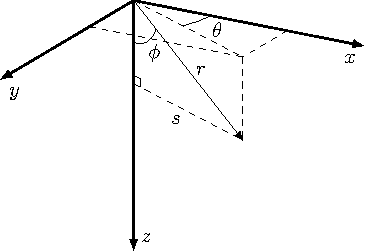
\includegraphics[width=8cm]{3d_coords.pdf}
  \caption{Spatial grid}
\end{figure}

\subsection{Domain}

Let the domain be defined as
\begin{equation}
  \begin{split}
    D = \big\{
    \vec{x} \in \RR^3 :\, &\xmin \leq \vec{x} \cdot \hat{x} \leq \xmax \\
    \mbox{ and } &\ymin \leq \vec{x} \cdot \hat{y} \leq \ymax \\
    \mbox{ and } &\zmin \leq \vec{x} \cdot \hat{z} \leq \zmax
    \big\}
  \end{split}
\end{equation}

Let the surface and bottom of the domain be denoted respectively by
\begin{align}
  S &= \left\{\vec{x_s} \in D: \vec{x_s} \cdot \hat{z} = 0 \right\} \\
  B &= \left\{\vec{x_b} \in D: \vec{x_b} \cdot \hat{z} = 0 \right\}
\end{align}

\subsection{Assumptions}
We assume that the scattering coefficient is constant over space; that the
primary difference in the optical effects of kelp and water is absorption, not
scattering.

\begin{itemize}
  \item Scattering constant (same for kelp/water)
\end{itemize}
  
\subsection{Table of variables}

\section{Asymptotics Motivation}
\subsection{Limitations of Discrete Ordinates}
\begin{itemize}
  \item All angles are coupled by integral
  \item GMRES is very memory-intensive.
  \item It's very CPU-intensive as well.
  \item It also might never converge!
  \item Especially if we start from zero.
\end{itemize}
  
\subsection{Advantages of Asymptotics}
\begin{itemize}
  \item Solve each angular problem independently
  \item Relatively computationally cheap
  \item Much lower memory cost
  \item Known number of operations
  \item Low and high accuracy available
\end{itemize}
  
\section{RTE Formulation}
  
\subsection{RTE: 1D}
Consider a fixed position $\vec{x}$ and direction $\vec{\omega}$ such that
$\vec{\omega} \cdot \hat{z} \neq 0$.

** Just call $\vec{x_0}$ a point, not a function. Call it the projection to the surface.

Let $\vec{l}(\vec{x}, \vec{\omega}, s)$ denote the linear path containing $\vec{x}$
with initial z coordinate given by
\begin{equation}
  z_0 =
   \begin{cases}
    0, & \vec{\omega} \cdot \hat{z} < 0 \\
    \zmax, & \vec{\omega} \cdot \hat{z} > 0
  \end{cases}
\end{equation}

Then,
\begin{equation}
  \vec{l}(\vec{x}, \vec{\omega}, s) = \frac{1}{\tilde{s}} (s\vec{x} + (\tilde{s} - s)\vec{x_0}(\vec{x}, \vec{\omega}))
\end{equation}

where
\begin{equation}
  \vec{x_0}(\vec{x}, \vec{\omega}) = \vec{x} - \tilde{s} \vec{\omega}
\end{equation}
is the origin of the ray, and 

\begin{equation}
  \tilde{s} = \frac{\vec{x} \cdot \hat{z} - z_0}{\vec{\omega} \cdot \hat{z}}
\end{equation}
is the path length from $\vec{x_0}(\vec{x}, \vec{\omega})$ to $\vec{x}$.

\subsection{Colloquial Description}
Denote the radiance at $\vec{x}$ in the direction $\vec{\omega}$ by $L(\vec{x}, \vec{\omega})$.
As light travels along $\vec{l}(\vec{x}, \vec{\omega}, s)$, interaction with the
medium produces three phenomena of interest:
\begin{enumerate}
  \item Radiance is decreased due to absorption.
  \item Radiance is decreased due to scattering out of the path to other
    directions.
  \item Radiance is increased due to scattering into the path from other
      directions.
\end{enumerate}

\subsection{IOPs}
These phenomena are governed by three inherent optical properties (IOPs) of the
medium.
The absorption coefficient $a(\vec{x})$ (units m$^{-1}$) defines the
proportional loss of radiance per unit length.
The scattering coefficient $b$ (units m$^{-1}$), defines the proportional loss
of radiance per unit length, and is assumed to be constant over space.

The volume scattering function (VSF) $\beta(\Delta): [0, \pi] \to \RR^+$ (units sr$^{-1}$) defines the
proportion of radiance scattered at an angle $\Delta$ from it's original
direction.
The VSF is normalized such that $\int_0^{\pi}\beta(\Delta)\,d\Delta = 1$.
The scattering coefficient $b$ can be considered the magnitude of the unnormalized VSF.

\subsection{Equation of Transfer}
Then, combining these phenomena, the Radiative Transfer equation along
$\vec{l}(\vec{x}, \vec{\omega})$ becomes
\begin{equation}
  \label{eqn:rte1d}
  \frac{dL}{ds}(\vec{l}(\vec{x}, \vec{\omega}, s), \vec{\omega})
  = -(a(\vec{x}) + b)L(\vec{x}, \vec{\omega})
  + b \int_{4\pi} \beta(|\vec{\omega} - \vec{\omega}'|) L(\vec{x})\, d\omega',
\end{equation}
where $\int_{4\pi}$ denotes integration over the unit sphere and
$|\vec{\omega}-\vec{\omega}'| = \cos^{-1}(\abs{\vec{\omega} - \vec{\omega}'})$.

\subsection{RTE: Vector}

Now, we have
\begin{align*}
  \frac{dL}{ds}(\vec{l}(\vec{x}, \vec{\omega}, s), \vec{\omega})
    &= \frac{d\vec{l}}{ds}(\vec{x}, \vec{\omega}, s) \cdot \nabla L(\vec{x, \vec{\omega}'}, \vec{\omega}) \\
    &= \vec{\omega} \cdot \nabla L(\vec{x}, \vec{\omega})
\end{align*}

Then, the general form of the Radiative Transfer Equation is
\begin{equation}
  \vec{\omega} \cdot \nabla L(\vec{x}, \vec{\omega})
  = -(a(\vec{x}) + b)L(\vec{x}, \vec{\omega})
  + b \int_{4\pi} \beta(|\vec{\omega} - \vec{\omega}'|) L(\vec{x}, \vec{\omega}')\, d\omega'
\end{equation}

or, equivalently,
\begin{equation}
  \vec{\omega} \cdot \nabla L(\vec{x}, \vec{\omega})
  + a(\vec{x})L(\vec{x}, \vec{\omega})
  = b \left(
    \int_{4\pi} \beta(|\vec{\omega} - \vec{\omega}'|) L(\vec{x}, \vec{\omega}')\, d\omega'
    - L(\vec{x}, \vec{\omega})
  \right)
\end{equation}

\section{Asymptotics}
\subsection{Substitute asymptotic series}
\newcommand{\Lasym}{L_0(\vec{x},\vec{\omega}) + b L_1(\vec{x},\vec{\omega}) + b^2 L_2(\vec{x},\vec{\omega}) + \cdots}
\newcommand{\Lasymp}{L_0(\vec{x},\vec{\omega}') + b L_1(\vec{x},\vec{\omega}') + b^2 L_2(\vec{x},\vec{\omega}') + \cdots}
\begin{align}
  L(\vec{x},\vec{\omega}) = \Lasym
\end{align}

Then, substituting the above into the RTE,

\begin{equation}
  \begin{split}
    \vec{\omega} \cdot \nabla \left[ \Lasym \right]
    &+ a(\vec{x}) \left[ \Lasym \right] \\
    &= b\Bigg(
      \int_{4\pi} \beta(\abs{\vec{\omega} - \vec{\omega}'})
      \left[ \Lasymp \right] \, d\vec{\omega}' \\
    &- \left[ \Lasym \right]
    \Bigg)
    \end{split}
\end{equation}

Now, grouping like powers of $b$, we have the decopled set of equations
\begin{align}
  \vec{\omega} \cdot \nabla L_0(\vec{x}, \vec{\omega}) + a(\vec{x})L_0(\vec{x}) &= 0 \\
  \vec{\omega} \cdot \nabla L_1(\vec{x}, \vec{\omega}) + a(\vec{x})L_1(\vec{x})
  &= \int_{4\pi} \beta(\abs{\vec{\omega} - \vec{\omega}'}) L_0(\vec{x}, \vec{\omega}')\,d\vec{\omega}' - L_0(\vec{x}, \vec{\omega}) \\ 
  \vec{\omega} \cdot \nabla L_2(\vec{x}, \vec{\omega}) + a(\vec{x})L_2(\vec{x})
  &= \int_{4\pi} \beta(\abs{\vec{\omega} - \vec{\omega}'}) L_1(\vec{x}, \vec{\omega}')\,d\vec{\omega}' - L_1(\vec{x}, \vec{\omega}) \\ 
  &\vdots \nonumber
\end{align}

\subsection{Boundary Conditions}

We use periodic boundary conditions in the $x$ and $y$ directions.
\begin{align}
  L\left((\xmin, y, z), \vec{\omega}\right) &= L\left((\xmax, y, z), \vec{\omega}\right) \\
  L\left((x, \ymin, z), \vec{\omega}\right) &= L\left((x, \ymax, z), \vec{\omega}\right)
\end{align}

In the $z$ direction, we specify a spatially uniform downwelling light just
under the surface of the water by a function $f(\vec{\omega})$.

* $\zmin$ could also be much lower, e.g. 5m.

Further, we assume that no upwelling light enters the domain from the bottom.
\begin{align}
  L(\vec{x_s}, \vec{\omega}) &= f(\omega) \mbox{ if } \vec{\omega} \cdot \hat{z} > 0\\ 
  L(\vec{x_b}, \vec{\omega}) &= 0 \mbox { if } \vec{\omega} \cdot \hat{z} < 0
\end{align}
 
\subsection{Rewrite as ODE along ray path}
For all $\vec{x}, \vec{\omega}$, let
\begin{align}
  \tilde{a}(s) &= a(\vec{l}(\vec{x}, \vec{\omega}), s), \\ 
  \frac{du_0}{ds}(s) + \tilde{a}(s) u_0(s) &= 0, u_0(0) = f(\vec{\omega})
\end{align}
Then,
\begin{align}
  u_0(s) = f(\omega) \exp\left(-\int_0^s \tilde{a}(s)\, ds\right), \\
  L_0(\vec{l}(\vec{x}, \vec{\omega},s), \vec{\omega}) = u_0(s)
\end{align}

\begin{align}
  g_n(s) = \int_{4\pi} \beta(\abs{\vec{\omega} - \vec{\omega}'})
  L_{n-1}(\vec{l}(\vec{x}, \vec{\omega'}, s), \vec{\omega}')\,d\vec{\omega}' - L_{n-1}(\vec{l}(\vec{x}, \vec{\omega}, s), \vec{\omega}) \\ 
  \frac{du_n}{ds}(s) + \tilde{a}(s)u_n(s) = g_n(s), u_n(0) = 0
\end{align}

Then,
\begin{align}
  u_n(s) = \int_0^sg_n(s')\exp\left( -\int_{s''}^{s'}\tilde{a}(s'')\,ds'' \right)\, ds' \\
  L_n(\vec{l}(\vec{x}, \vec{\omega}, s), \vec{\omega}) = u_n(s)
\end{align}

\subsection{Solve ODE as 1st order linear via I.F.}

\section{Physical Interpretation}

\section{Numerical Implementation}

Following is a description of the uniform, rectangular spatial-angular grid used
in the numerical implementation of this model.
It is assumed that all simulated quantities are constant over the interior of a
grid cell.
The following indices are assigned to each dimension:
\begin{align}
  x &\to i \\
  y &\to j \\
  z &\to k \\
  \theta &\to l \\
  \phi &\to m
\end{align}

Then, the center of a generic grid cell will be denoted as
$(x_i,y_j,z_k,\theta_l,\phi_m)$, and the boundaries between adjacent grid cells
will be referred to as \textit{edges}.
The number of grid points in each dimension are denoted by $n_x$, $n_y$, $n_z$,
$n_\theta$, and $n_\phi$, with uniform spacings $dx$, $dy$, $dz$, $d\theta$, and
$d\phi$ between adjacent grid points.
Each dimension has the same number of edges as cells.
One-indexing will be employed throughout this document.
\subsection{Spatial Grid}
\begin{figure}[H]
  \centering
  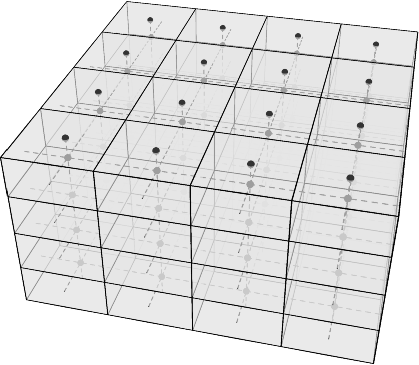
\includegraphics[width=8cm]{spatialgrid.pdf}
  \caption{Spatial grid}
  \label{fig:spatial_grid}
\end{figure}

\begin{align}
  dx &= \frac{x_{\max}-x_{\min}}{n_x} \\ 
  dy &= \frac{y_{\max}-y_{\min}}{n_y} \\ 
  dz &= \frac{z_{\max}-z_{\min}}{n_z}
\end{align}

Then,
\begin{align}
  x_i &= (i-1/2)dx \\
  y_j &= (j-1/2)dy \\
  z_k &= (k-1/2)dz
\end{align}

\subsection{Surface Radiance}
Note that $0$ is not stored as a grid center in any spatial dimension.
Radiance values for the surface boundary condition are stored
separately as the four-dimensional array $\left(f_{ijlm}\right)$.

\subsection{Angular Grid}
\begin{figure}[H]
  \centering
  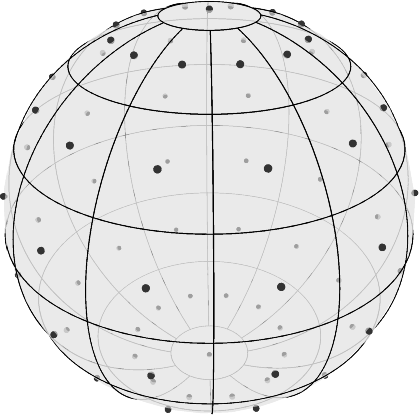
\includegraphics[width=8cm]{angulargrid.pdf}
  \caption{Angular grid}
  \label{fig:angular_grid}
\end{figure}

As shown in Figure \ref{fig:angular_grid}, $\phi=0$ and $\phi=\pi$ are treated
separately.
These grid cells are referred to as poles.
Accordingly, we have 
\begin{align}
  \phi_1 &= 0, \\
  \phi_{n_\phi} &= \pi.
\end{align}

Meanwhile, $\theta$ is similar to the spatial dimensions in that its extreme
values are not grid centers.

Then,
\begin{align}
  d\theta &= \frac{2\pi}{n_\theta}, \\
  d\phi &= \frac{\pi}{n_\phi-1}.
\end{align}

Then,
\begin{align}
  \theta_l = (l-1) d\theta, \\
  \phi_m = (m-1) d\phi
\end{align}

\subsubsection{Storing pole values}
We store pole values in the $(1,1)$ and $(1,n_\phi)$ positions.

\subsection{Angular Quadrature}
We assume that all quantities are constant within a spatial-angular grid cell.
We therefore employ the midpoint rule for both spatial and angular integration.

** Need to define $\mathcal{X}$ in this context, I think.

** Is $d\theta$, etc. for both differential and grid spacing confusing?

\begin{align}
  \int_{4\pi} f(\vec{\omega})\,d\vec{\omega} &= \int_0^{2\pi} \int_0^{\pi} f(\theta, \phi) \sin(\phi)\, d\phi\, d\theta \\
  &\mbox{**Need to deal with poles separately**} \\
                                             &= \int_0^{2\pi}\int_0^{\pi} \sum_{l=1}^{n\theta}\sum_{m=1}^{n\phi}f_{lm}\mathcal{X}_l(\theta) \mathcal{X}_m(\phi) \sin(\phi)\, d\phi\, d\theta \\
                                             &= \sum_{l=1}^{n\theta}\sum_{m=1}^{n\phi}f_{lm}\int_{\theta_l}^{\theta_{l+1}}\int_{\phi_m}^{\phi_{m+1}} \sin(\phi)\, d\phi\, d\theta \\
                                             &= d\theta\sum_{l=1}^{n\theta}\sum_{m=1}^{n\phi} f_{lm}\int_{\phi_m}^{\phi_{m+1}} \sin(\phi)\, d\phi \\
                                             &= d\theta\sum_{l=1}^{n\theta}\sum_{m=1}^{n\phi} f_{lm}\left( \cos(\phi_m-d\phi/2)-\cos(\phi_m+d\phi/2) \right) \\
\end{align}

\subsection{Ray Tracing Algorithm}
\subsubsection{Extract values along path}
- Path spacing ($s$)

In order to evaluate a path integral through the previously described grid, it
is first necessary to construct a one-dimensional piecewise constant integrand
which is discontinuous at unevenly spaced points corresponding to the
intersections between the path and edges in the spatial grid.

Consider a grid center $\vec{x_1} = (x_1,y_1,z_1)$ and a corresponding path $\vec{l}(\vec{x_1}, \vec{\omega}, s)$.
To find the location of discontinuities in the itegrand, we first calculate the
distance from its origin, $\vec{x_0}(\vec{x_1}, \vec{\omega}) = (x_0, y_0, z_0)$ to grid edges in each dimension
separately.


** THIS NOTATION IS OVERLOADED **

Given
\begin{align}
  x_i &= x_0 + s_i^x/\tilde{s}(x_1-x_0) \\
  y_j &= y_0 + s_j^y/\tilde{s}(y_1-y_0) \\
  z_k &= z_0 + s_k^z/\tilde{s}(z_1-z_0) \\
\end{align}

we have
\begin{align}
  s_i^x &= \tilde{s}\frac{x_i-x_0}{x_1-x_0} \\
  s_i^y &= \tilde{s}\frac{y_i-y_0}{y_1-y_0} \\
  s_i^z &= \tilde{s}\frac{z_i-z_0}{z_1-z_0} \\
\end{align}

Then, move to the adjacent grid cell in the dimension which requires the shortes
step to reach an edge. Save $ds$ of the path through this cell. Also save abs.
coef. and source.
** Definitely needs more work**

- absorption coefficient ($\tilde{a}(s)$)

- effective source ($g_n(s)$)
0
\subsubsection{Ray integral}

Let
\begin{align}
  g_n(s) &= \sum_{i=1}^{N-1}g_{ni}\mathcal{X}_i(s) \\
  \tilde{a}(s) &= \sum_{i=1}^{N-1}\tilde{a}_{i}\mathcal{X}_i(s) \\
\end{align}

and
\begin{equation}
  \mathcal{X}_i(s) = \begin{cases}
    1, & a_I \leq s < s_{i+1} \\
    0, & \mbox{otherwise}
    \end{cases}
\end{equation}

and $\left\{s_i\right\}_{i=1}^N$ is increasing.

Let $ds_i = s_{i+1} - s_i$.

Let $\hat{i}(s) = \min\left\{ i \in \{1,\ldots,N\} : s_i>s \right\}$.
Let $\tilde{d}(s) = s_{\hat{i}(s)}-s$.

We have $s_1 = 0$ and $s_N = \tilde{s}$.


\begin{align}
  u_n(\tilde{s}) &= \int_0^{\tilde{s}}g_n(s')\exp\left( -\int_{s''}^{s'}\tilde{a}(s'')\,ds'' \right)\, ds' \\
  &= \int_0^{s_N} \sum_{i=1}^{N-1}g_{ni}\mathcal{X}_i(s') \exp\left( -\int_{s''}^{s'}\sum_{j=1}^{N-1}\tilde{a}_{j}\mathcal{X}_j(s'')\,ds'' \right)\, ds' \\
  &= \sum_{i=1}^{N-1}g_{ni}\int_0^{s_N} \mathcal{X}_i(s') \exp\left( -\sum_{j=1}^{N-1}\tilde{a}_{j}\int_{s''}^{s'}\mathcal{X}_j(s'')\,ds'' \right)\, ds' \\
  &= \sum_{i=1}^{N-1}g_{ni}\int_{s_i}^{s_{i+1}}  \exp\left(-\tilde{a}_{\hat{i}(s')-1}\tilde{d}(s') -\sum_{j=\hat{i}(s')}^{N-1}\tilde{a}_{j}ds_j\right)\, ds' \\
  &= \sum_{i=1}^{N-1}g_{ni}\int_{s_i}^{s_{i+1}}  \exp\left(-\tilde{a}_{i}(s_{i+1}-s') -\sum_{j=i+1}^{N-1}\tilde{a}_{j}ds_j\right)\, ds'
\end{align}

Let
\begin{equation}
  b_i = -\tilde{a}_{i}s_{i+1} - \sum_{j=i+1}^{N-1}\tilde{a}_{j}ds_j.
\end{equation}

Then,
\begin{equation}
  u_n(\tilde{s}) = \sum_{i=1}^{N-1}g_{ni}\int_{s_i}^{s_{i+1}}  \exp\left(\tilde{a}_{i}s' +b_i\right)\, ds'
\end{equation}

Let
\begin{align}
  d_i &= \int_{s_i}^{s_{i+1}}  \exp\left(\tilde{a}_{i}s' +b_i\right)\, ds' \\
    &= \begin{cases}
    ds_i \exp(b_i), & \tilde{a} = 0 \\
      \left( \exp(\tilde{a}_i s_{i+1}) - \exp(\tilde{a}_i s_i) \right)/\tilde{a}_i, & \mbox{otherwise}
    \end{cases}
\end{align}

Then,
\begin{equation}
  u_n(\tilde{s}) = \sum_{i=1}^{N-1} g_{ni}d_i
\end{equation}

\end{document}
